\subsection{Prime Time Ratio}
\label{subsec:prime-time}

%We reaffirm the importance of measuring performance during the prime-time peak hours, and urge the FCC to revisit and standardize the measurement and interpretation of \textbf{prime-time ratio}. 
%we show through our analysis that the \textbf{prime-time ratio
%(ratio of average data rate during prime time hours to non prime time hours)
%does not follow the conventional definition stated by the FCC.

In section ~\ref{sec:methodology}, we established the importance of measuring behavior during prime time hours. To reiterate, the prime time hours as defined by the FCC is the period between 7:00 PM -- 11:00 PM on weeknights when the network is under peak load~\cite{fcc2014measuring-broadband}. \todo{The first occurrence of this definition was ... should this be in methodology?? }

Our analysis of the peak usage in figure~\ref{fig:TS-data-rate-daily} motivated us to revisit this definition. We observed that in our dataset the four hour period 8:00 PM -- 12:00 AM is a much better indicator of prime-time hours than the FCC's original definition over both sets of data. This discrepancy could be limited to high tier households only, or it could imply that due to the flexibility of video-on-demand, consumers across the country are opting for a later time to watch video.

\begin{itemize}
\itemsep0em 
\item Figure ~\ref{fig:TS-prime-time-ratio}
\item 8p - 12a shows a higher prime-time ratio than 7p - 11p (as stated by FCC) in the Comcast data set. The curve in convex, i.e. there is only one peak time in a day.
\item Distribution of prime time ratios over control and test set is very similar
\item The average prime-time ratio for control sets is consistently higher than test set
\item Test set has 10\% lower PT than control set
\item Diurnal pattern shows high ratio for 5 weekdays, and low ratio on weekends.
\item Also easy to see Thanksgiving, black friday, Christmas, etc. holidays
\end{itemize}



%\sg{can also include PT table from ppt if worth it -- table shows the "no dip" pattern similar to time series in first subsection.}


%%%%%%%%%%%%%%%%%%%%%%%%%%%%%%%%%%%%%%%%%%%%%%%%%%%%%%%%%%%%%%%%%%%%%

\begin{figure}[ht!]
\begin{minipage}{\linewidth}
\centering
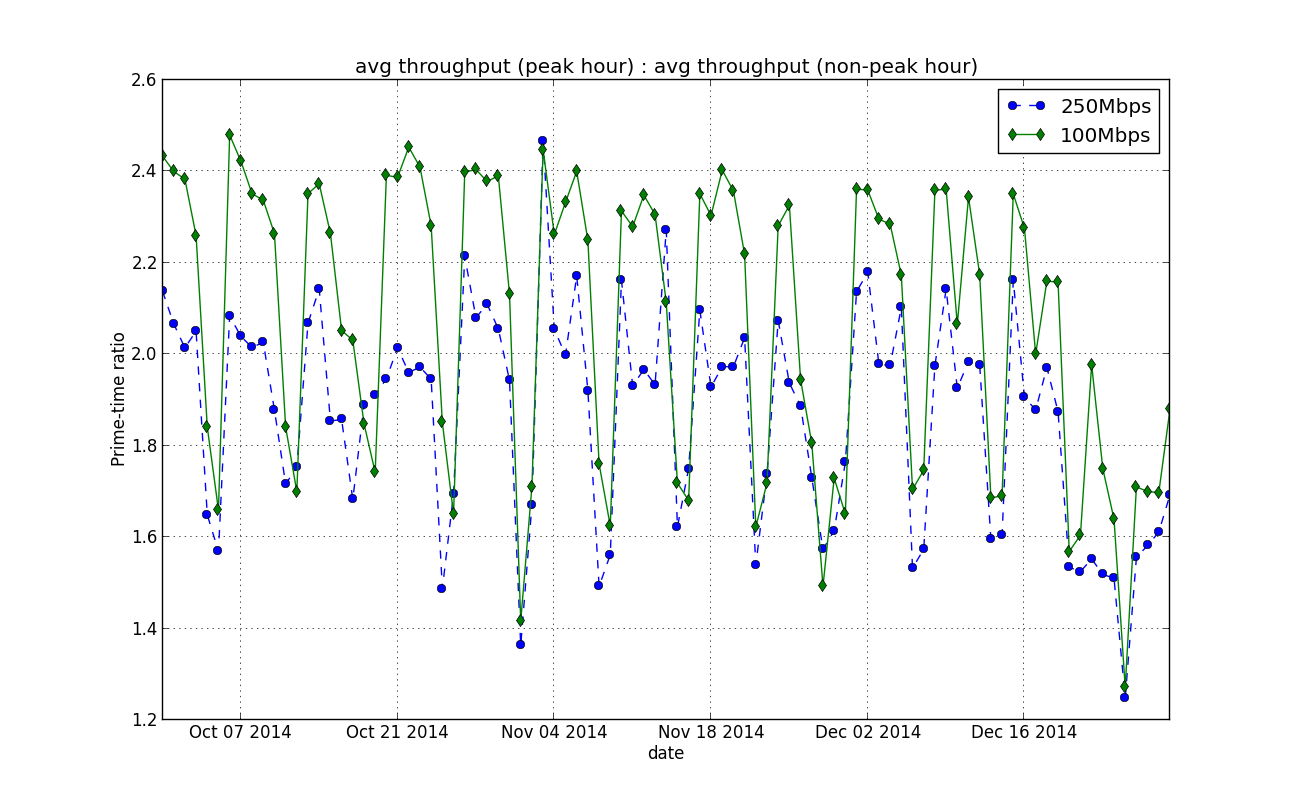
\includegraphics[width=\linewidth]{figures/prime-time-ratio-by-date[replace].png}
\caption{Prime Time ratio showing weekly pattern + differences during holiday periods (Thanksgiving, Christmas)}
%http://riverside.noise.gatech.edu:8083/separated/full/prime-time-ratio-by-date.png
\label{fig:TS-prime-time-ratio}
\end{minipage}
\end{figure}

%%%%%%%%%%%%%%%%%%%%%%%%%%%%%%%%%%%%%%%%%%%%%%%%%%%%%%%%%%%%%%%%%%%%%



% \sg{ http://riverside.noise.gatech.edu:8083/separated/full/cdf-prime-time-ratio-per-device.png not needed ? }



\begin{itemize}
\itemsep0em 
\item Figure ~\ref{fig:TS-prime-time-ratio}
\item 8p - 12a shows a higher prime-time ratio than 7p - 11p (as stated by FCC) in the Comcast data set. The curve in convex, i.e. there is only one peak time in a day.
\item Distribution of prime time ratios over control and test set is very similar
\item The average prime-time ratio for control sets is consistently higher than test set
\item Test set has 10\% lower PT than control set
\item Diurnal pattern shows high ratio for 5 weekdays, and low ratio on weekends.
\item Also easy to see Thanksgiving, black friday, Christmas, etc. holidays
\end{itemize}
